\documentclass[10pt,conference,compsocconf]{IEEEtran}

\usepackage{hyperref}
\usepackage{graphicx}	% For figure environment
\usepackage{amsfonts, amsmath}
\usepackage{multirow}
\usepackage[caption=false,font=footnotesize]{subfig}
\usepackage{subcaption}
\usepackage{caption}


\makeatother

\begin{document}
\title{Measuring the effectiveness of quantization on SpeedyQ and vanilla Q-learning}

\author{
  Killian Didierjean, Charles Mercier, Mathis Hage,\\
  \textit{EPFL --- School of Computer and Communication Sciences}
}

\maketitle

\begin{abstract}
 Reinforcement Learning is today widely used to solve a variety of problems. In particular, Q-learning is a very popular method allowing one to learn a policy without needing a predefined model of the environment. However, it can rapidly require a lot of memory space to function. In this paper, we study quantization of the Q-table : we will see that this method can lead up to at least 8 times less space used, without any significant loss in results quality.
\end{abstract}

\section{Introduction}

    Since the formal introduction of \textit{Temporal Difference (TD) Learning} by Richard S. Sutton in his 1988 paper \cite{suttonTDLearning}, the field has seen constant improvements over the years, with the discoveries and enhancements of algorithms that are becoming always more efficient. A heavily sought after subclass of TD learning algorithms are the ones used to estimate the Q-function of a reinforcement learning (RL) task, known as \textit{Q-learning} algorithms.

    In addition to the original vanilla Q-learning algorithm, Ghavamzadeh et al. for example introduced a faster version of the vanilla $Q$-learning called \textit{SpeedyQ} in 2011. 
    
    Unfortunately, Q-learning can quickly require a lot of computational power. Some work like for example the 2022 paper by S. Krishnan et al. \cite{krishnan2022quarlquantizationfastenvironmentally} discuss the use of \textit{quantization} for better efficiency in RL tasks.

    Our contribution will be to compare two versions of $Q$-learning : vanilla and \textit{SpeedyQ} and, more specifically, to see how they both behave under quantization of the Q-table at training time. Informally : up to what point can we discretize the possible values that a Q-table entry can take, while still obtaining quality results ?

\section{Background and Setup}

    In this section, we recall the basics of Q-learning and \textit{SpeedyQ}, as it is done in \cite{weng2019momentumbasedacceleratedqlearning}, before exposing our training-time quantization setup, taken from \cite{gupta2015}.

    \subsection{Q-learning}

        The problem takes place as a standard reinforcement learning problem, where an agent interacts with its environment. This environment is modeled as a discrete-time discounted \textit{Markov Decision Process} (MDP), which is a quintuple $(\mathcal{S}, \mathcal{A}, P, R, \gamma)$ where $\mathcal{S}$ is the state space ; $\mathcal{A}$ is the state of actions ; $P$ is the probability function for state transitions :

            $$
            \begin{aligned}
                P\colon \mathcal{S} \times \mathcal{A} \times \mathcal{S} & \rightarrow [0, 1] \\
                (s_i, a, s_{i-1}) &\mapsto \mathbb{P}(s_i | a, s_{i-1})
            \end{aligned}
            $$
            
            i.e. the transition probability to a certain state given an action as well as the previous state ; $R$ is the reward function : $R: \mathcal{S} \times \mathcal{A} \rightarrow \text{Im}(R)$ where $\text{Im}(R) \subset \mathbb{R}$ is bounded ;
            and $\gamma$ is the discount factor.

        A \textit{Q-function} or \textit{Q-table} $Q: \mathcal{S} \times \mathcal{A} \to \mathbb{R}$ 
        is defined as the expected future reward given that we are in a fixed state and following some action. The main challenge of Q-learning is finding an efficient way to learn the Q-function $Q^*$ characterizing the optimal choices to make at each step. Vanilla Q-learning is simply an analogy with gradient descent ; if $Q_k$ is the state of the $Q$ function at step $k$, then :

        \begin{equation}
            Q_{k+1}(s, a) = Q_k(s, a) - \alpha_k (Q_k(s, a) - \mathcal{T}_k Q_k(s, a) )
            \label{eq:vanilla_q_learning_update}
        \end{equation}

        Where $\alpha_k \in [0, 1[$ is the learning rate at step $k$, and where we introduced the \textit{empirical Bellman operator} $\mathcal{T}_k$ as :
        
        \begin{equation}
         \mathcal{T}_k Q(s, a) = R(s, a) + \gamma \max_{a' \in A(s')} Q_k (s', a').
        \end{equation}
        
        $s'$ is the state attained by performing action $a$ at state $s$, and $A(s')$ is the set of states accessible from $s'$.

        
    \subsection{Speedy Q-Learning}

        This is an upgraded version of Q-Learning with momentum inspired by Nesterov’s accelerated gradient (NAG) \cite{nesterov1983method}. The update step is :

        \begin{equation}
        Q_{k+1} = Q_k + \alpha_k(\mathcal{T}_k Q_{k-1} - Q_k) + (1-\alpha_k)(\mathcal{T}_k Q_k - \mathcal{T}_k Q_{k-1})
        \label{eq:speedy_q_equation}
        \end{equation}\\
        where $\alpha_k$ is the learning rate. Speedy-Q adds the term $(1-\alpha_k)(\mathcal{T}_k Q_k - \mathcal{T}_k Q_{k-1})$ which contains the momentum's history for faster convergence
        
    
    \subsection{Quantization of the Q-table}

        To reduce the space taken by the Q-table in memory, one can introduce training-time quantization.

    Suppose we have a Q-table with values in $[v_\text{min}, v_\text{max}]$, and that we want to use quantization on $b$ bits. The goal is to reduce all the values in the interval $[v_\text{min}, v_\text{max}]$ to a discrete set of values $2^b - 1$, uniformly spaced with a step of $\Delta := (v_{\max} - v_{\min})/(2^b - 1)$. A value $v$ is rounded with probability proportional to its fractional position within the bin:
        
        \begin{equation}
            Q_b^{\text{stoch}}(v) =
            \begin{cases}
                \lceil p \rceil \cdot \Delta + v_{\min}
                    & \text{with probability } p - \lfloor p \rfloor \\
                \lfloor p \rfloor \cdot \Delta + v_{\min}
                    & \text{otherwise}
            \end{cases}
        \end{equation}\\
        
        where $p = (v - v_{\min}) / \Delta$. Therefore, the Q-table now only stores the \textit{index} of the value, i.e. $\lfloor p \rfloor$ or $\lceil p \rceil$, respectively.
        
        We chose this scheme (\textit{stochastic rounding}) in opposition to the deterministic \textit{round-to-nearest} version because the former is unbiased: $\mathbb{E}[Q_b^{\text{stoch}}(v)]
        = v$ \cite{gupta2015}.
        
        It is clear that with quantization, there is now a tradeoff between memory improvements and accuracy of the results. We will see its impact empirically.

        % \paragraph{Round-to-nearest}
        
        % The quantized value of $v$ is:
        
        % \begin{equation}
        %     Q_b(v) = \left\lfloor \frac{v - v_{\min}}{\Delta} + \frac{1}{2}
        %     \right\rfloor \cdot \Delta + v_{\min}
        %     \label{eq:quantization}
        % \end{equation}\\

        %\paragraph{Stochastic rounding}

        \section{Experiments}

        We perform Q-learning tasks on Gymnasium's discretized Cartpole environment \cite{towers2025gymnasiumstandardinterfacereinforcement}. The agent's objective is to maintain an unstable pole standing on a cart for as long as possible. To this end, it can either push the cart left or right. The total number of dimensions of the problem is 4.
        
        The training follows an $\varepsilon$-greedy approach. For both algorithms, the hyperparameters (i.e. $\varepsilon$ and $\alpha$) were tuned manually, seeking the best possible results in average. Precisions are available in the appendix. We also recall that the maximum reward the agent can accumulate in Cart Pole is 500. For faster convergence, we inflict a 100 points penalty when the agent fails. Moreover, training is done by averaging 16 runs over different seeds (characterizing randomness) to ensure quality of results.

        \subsection{Memory usage}

        The main objective of quantization is to reduce the memory taken by the Q-table. For a fixed number of bins, lowering the number of bits per entry shrinks the table by a factor that is linear with respect to the bit-width as shown in Tab. (\ref{tab:mem_usage}). For example if 8-bits quantization appeared to be effective, it would lead to 8 times less memory used for vanilla and 4 times less memory used for \textit{SpeedyQ} (notice that \textit{SpeedyQ} needs twice as much memory as vanilla : this is because it retains the old Q-table for momentum). This would be quite significant.

        \begin{table}[]
        \centering
        \begin{tabular}{|l|c|c|c|}
        \hline
        \textbf{Config} & \textbf{Theory} & \textbf{Vanilla} & \textbf{SpeedyQ} \\ \hline
        2-bit           & 800             & 3200             & 6400             \\
        4-bit           & 1600            & 3200             & 6400             \\
        8-bit           & 3200            & 3200             & 6400             \\
        16-bit          & 6400            & 6400             & 12800            \\
        32-bit          & 12800           & 12800            & 25600            \\ 
        Full precision  & 25600           & 25600            & 51200            \\ \hline
        \end{tabular}
        \caption{Memory usage (in bytes) of the Q-tables of the algorithms. Theory corresponds to the theoretical size of a single Q-table, while Vanilla and \textit{SpeedyQ} measured experimentally.}
        \label{tab:mem_usage}
        \end{table}

        \subsection{Computation time}

        Since with quantization the number of possible values is now discreet, it isn't unreasonable to expect faster training runtime. However, to go from episode $k$ to $k+1$, the Q-table update formulas still require converting the index back to the corresponding floating point value : the conversions from index to float and then from float to index add an extra computational overhead. Tab. (\ref{tab:computation_time}) clearly shows that this overhead shatters any hope of time complexity improvements. Moreover, it also underlines that \textit{SpeedyQ} runs faster than the vanilla version in general. We will see that this is not necessarily a good sign, as the update formula of \textit{SpeedyQ} involves more calculations than vanilla : one would have imagined the opposite to be true.

        \begin{table}[t]
        \centering
        \begin{tabular}{|l|cc|cc|}
        \hline
        \multirow{2}{*}{\textbf{Config}} & \multicolumn{2}{c|}{\textbf{Vanilla}} & \multicolumn{2}{c|}{\textbf{SpeedyQ}} \\ \cline{2-5}
                                         & \multicolumn{1}{c|}{\textbf{Mean}} & \textbf{Std} & \multicolumn{1}{c|}{\textbf{Mean}} & \textbf{Std} \\ \hline
        4-bit                            & \multicolumn{1}{c|}{38.41} & 3.22 & \multicolumn{1}{c|}{10.30} & 4.69 \\ \hline
        8-bit                            & \multicolumn{1}{c|}{47.02} & 1.40 & \multicolumn{1}{c|}{40.31} & 5.07 \\ \hline
        16-bit                           & \multicolumn{1}{c|}{43.57} & 1.50 & \multicolumn{1}{c|}{35.16} & 3.82 \\ \hline
        Full precision                   & \multicolumn{1}{c|}{30.16} & 0.58 & \multicolumn{1}{c|}{26.51} & 2.65 \\ \hline
        \end{tabular}
        \caption{Computation time (in seconds) of the training, on a Apple Mac M1 pro with joblib multiprocessing.}
        \label{tab:computation_time}
        \end{table}

    

        \subsection{Convergence rate}

        Even though quantization achieves better memory usage, we talked earlier about the tradeoff that one deals with when introducing it. Fig. (\ref{fig:rewards_over_time}) shows the speed of convergence of the two methods, for various quantization setups.

        \begin{figure}[t]
            \centering
        
            \subfloat[]{%
                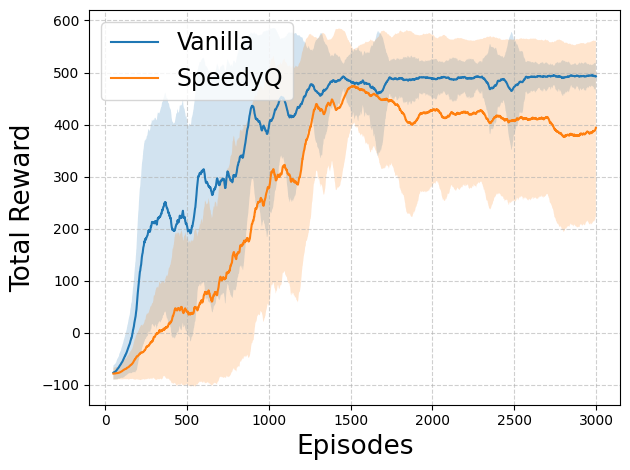
\includegraphics[width=0.45\linewidth]{res/reward/reward_full_precision.png}
                \label{fig:rewards_a}
            }
            \hfill
            \subfloat[]{%
                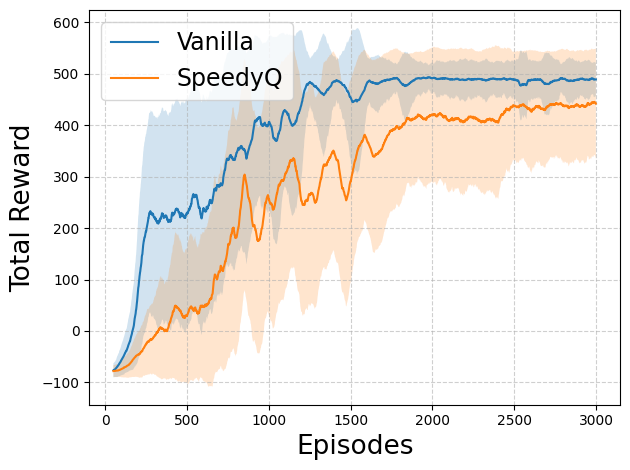
\includegraphics[width=0.45\linewidth]{res/reward/reward_16_bits.png}
                \label{fig:rewards_b}
            }
        
            \vspace{2mm}
        
            \subfloat[]{%
                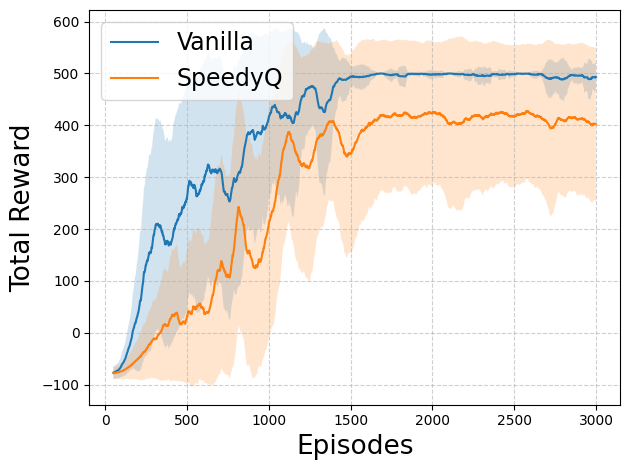
\includegraphics[width=0.45\linewidth]{res/reward/reward_8_bits.png}
                \label{fig:rewards_c}
            }
            \hfill
            \subfloat[]{%
                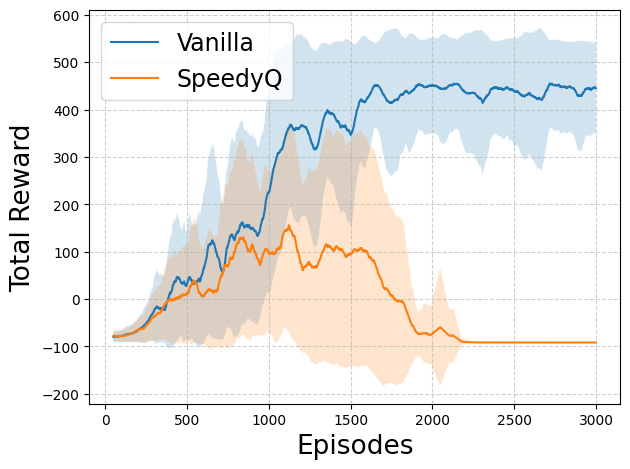
\includegraphics[width=0.45\linewidth]{res/reward/reward_4_bits.png}
                \label{fig:rewards_d}
            }
        
            \caption{Reward over time for both algorithms (3000 episodes), with (a) full precision, and (b), (c), (d) quantization with 16, 8 and 4 bits respectively. Results are shown as a moving average of window size 50 over the training results for 16 different seeds (with the standard deviation shown as well).}
            \label{fig:rewards_over_time}
        \end{figure}

        The first observation to be made is the most obvious one : even in the full precision case (Fig \ref{fig:rewards_over_time}.a), \textit{SpeedyQ} performs worse than vanilla. The latter almost always converges to an optimal configuration (i.e. leading to 500 points) in approximately 1500 episodes, while the former does not always reach such a configuration, and is quite noisy. With quantization enabled, we can see that both algorithms maintain their initial results in average, but with more and more variance as the number of bits goes down. When reaching 4 bits, \textit{SpeedyQ} collapses completely. The vanilla version seem to converge extremely well even with quantization, especially with 8 bits.

        \subsection{Success rate}

        Related to the preceeding section, another important metric we can look at is the \textit{success rate}, which we define to be the rate of runs that have attained 490 (98 \% of 500) points among the last 150 runs. Results are visible in Tab. (\ref{tab:cartpole_success_rate}).

        \begin{table}[h]
        \centering
        \begin{tabular}{|l|cc|cc|}
        \hline
        \multirow{2}{*}{\textbf{Config}} & \multicolumn{2}{c|}{\textbf{Vanilla}} & \multicolumn{2}{c|}{\textbf{SpeedyQ}} \\ \cline{2-5}
                                         & \multicolumn{1}{c|}{\textbf{Succeeded}} & \textbf{Rate} & \multicolumn{1}{c|}{\textbf{Succeeded}} & \textbf{Rate} \\ \hline
        4-bits                            & \multicolumn{1}{c|}{7/16}  & 43.8\% & \multicolumn{1}{c|}{0/16} &  0.0\% \\ \hline
        8-bits                            & \multicolumn{1}{c|}{11/16} & 68.8\% & \multicolumn{1}{c|}{7/16} & 43.8\% \\ \hline
        16-bits                           & \multicolumn{1}{c|}{12/16} & 75.0\% & \multicolumn{1}{c|}{7/16} & 43.8\% \\ \hline
        Full precision                   & \multicolumn{1}{c|}{13/16} & 81.2\% & \multicolumn{1}{c|}{7/16} & 43.8\% \\ \hline
        \end{tabular}
        \caption{Success rate of the algorithms across 16 seeds.}
        \label{tab:cartpole_success_rate}
        \end{table}
        
        Here, observe that for a given number of bins, the success rate of the Vanilla approach degrades as quantization with fewer and fewer bits is introduced, indicating slightly slower convergence each time. On the other hand, Speedy-Q fails to produce any results at 4-bit precision and consistently underperforms across 8-bit, 16-bit, and full precision settings.

         \subsection{Training Error}

        \begin{figure}[t]
            \centering
        
            \subfloat[]{%
                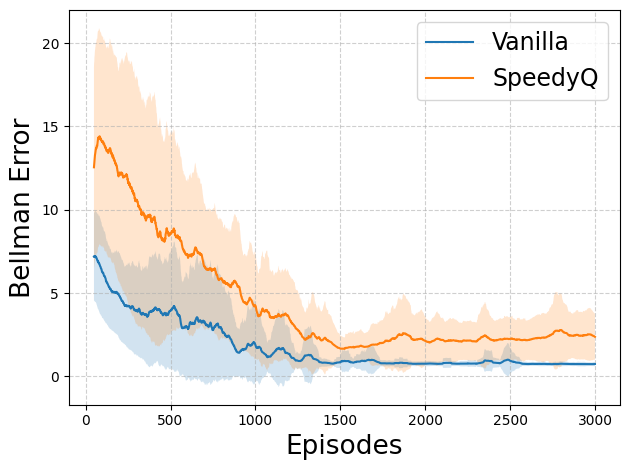
\includegraphics[width=0.45\linewidth]{res/bellman_error/error_full_precision.png}
                \label{fig:a}
            }
            \hfill
            \subfloat[]{%
                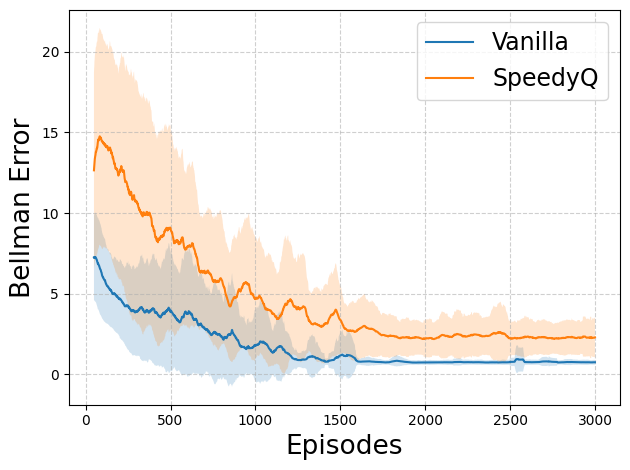
\includegraphics[width=0.45\linewidth]{res/bellman_error/error_16_bits.png}
                \label{fig:b}
            }
        
            \vspace{2mm}
        
            \subfloat[]{%
                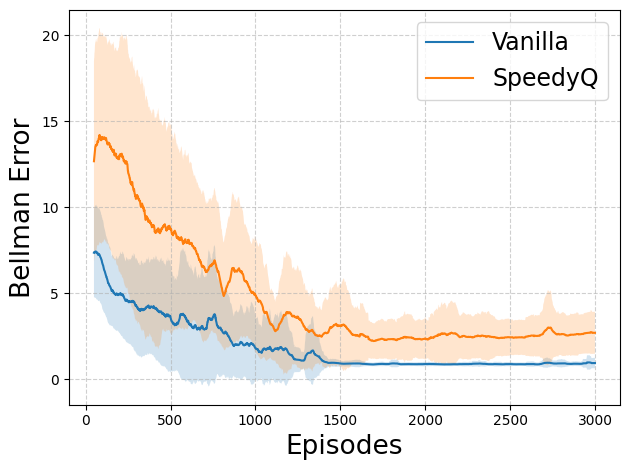
\includegraphics[width=0.45\linewidth]{res/bellman_error/error_8_bits.png}
                \label{fig:c}
            }
            \hfill
            \subfloat[]{%
                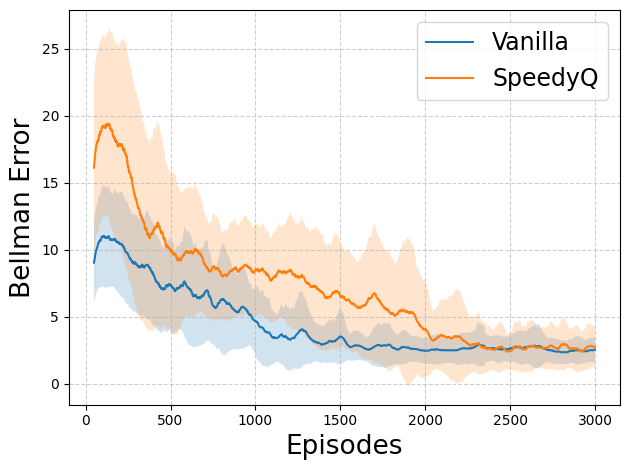
\includegraphics[width=0.45\linewidth]{res/bellman_error/error_4_bits.png}
                \label{fig:d}
            }
        
            \caption{Bellman absolute error over time for both algorithms (3000 episodes), with (a) full precision, and (b), (c), (d) quantization with 16, 8 and 4 bits respectively. Results are shown as a moving average of window size 50 over the training results for 16 different seeds (with the standard deviation shown as well).}
            \label{fig:bellman_error}
        \end{figure}

        Fig. (\ref{fig:bellman_error}) shows the Bellman absolute error of the runs, which measures how far the Q-table is from equilibrium, defined as $|\Delta_t| = \left| Q(s_t, a_t) - \left( r_t + \gamma \max_{a} Q(s_{t+1}, a) \right) \right|$. The plots confirm the trend we saw in the previous sections : the error for the quantized vanilla version follows the trend of the full precision version, even though a bit more slowly, while \textit{SpeedyQ} is less accurate, with a lot more noise.
        

        We can see this as follows : while \textit{SpeedyQ} was proven to be better in the \textit{synchronous} setting, it is the \textit{asynchronous} implementation that is more used in practice (and it is the case for us). Moreover, it is clear that Cart Pole is a very unforgiving game : if the momentum causes \textit{SpeedyQ} to overshoot by a tiny bit, the game ends and a severe penalty is inflicted to the agent. This effect is clearly amplified with quantization, as the memory that \textit{SpeedyQ} possesses looses even more precision. In general, this underlines the more unstable nature of \textit{SpeedyQ} : changing the randomness seed impacts the results significantly.

        On the other hand, the vanila implementation shows remarkable robustness under quantization, with the 8-bits case being particularly notable.


        \section{Conclusion and further studies}

        Our study allowed us to have a better feel of the effect of quantization on different Q-learning algorithms. Notably, the vanilla implementation performs extremely well in this setting, and we saw that with as much as 8 times less bits than for the full precision case, we can achieve excellent results in almost the same amount of training episodes. The \textit{SpeedyQ} case is less impressive : its memory-based nature makes it less resistant to the precision loss that quantization introduces, even though it can still be used if accepting less accurate results.

        Overall, we retain from this that training-time quantization is a very interesting tool for memory optimization even though it comes at a certain cost. But this cost may, in a well-thought setting, exclude the quality-of-the-results metric, which is an extremely valuable point. 

        To improve memory management even more, other points would deserve further study. In fact, the savings on the per-entry size introduced by our quantization is only a constant factor, while the number of entries grows exponentially as $\#\text{actions} \cdot \#\text{bins}^d$, with $d$ the dimension. Moreover, looking at Fig. (\ref{fig:visitation heat map}), only $7\%$ of the Q-table cells are ever visited, and the top $2.5\%$ of cells account for $99\%$ of all visits which shows the agent's experience is heavily concentrated in a small region of the discretized space. By adding for example dynamic allocation, one could theoretically obtain a table that is 44 times smaller than ours. These savings could be of great use for instance in edge computing applications, where storing a dense high-resolution table would not be possible.

        \begin{figure}[t]
            \centering
             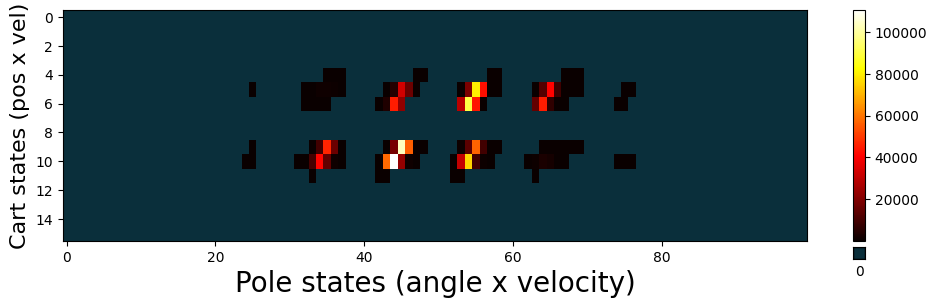
\includegraphics[width=0.85\linewidth]{res/state_visitation/state_visitation_8bit_heatmap.png}
           
        
            \caption{Visitation counts of trained Vanilla agent with 8-bits quantization.}
            \label{fig:visitation heat map}
        \end{figure}

        \appendix

        \subsection{Choice of Parameters}
        
        In addition to the discretization of the environment space, which is non-trivial, one also has to tune the algorithms' hyperparameters.
        
        \subsubsection{Environment Discretization}
        
        The CartPole environment returns a 4-dimensional continuous state vector. Our binning strategy roughly reflects the importance of each parameter : the pole angle $\theta$ and angular velocity $\dot{\theta}$ are critical, while the position of the cart $x$ as well as its velocity $\dot{x}$ are less important, and can tolerate a less precise discretization. Therefore, our choices are summarized in the table below.

        \begin{table}[h]
        \centering
        \begin{tabular}{|c|c|c|c|c|}
        \hline
        \textbf{Variable} & \textbf{Physical Range} & \textbf{ Practical Range } & \textbf{Bins}\\ \hline
        Cart position $x$ & $(-4.8, 4.8)$ & $(-4.8, 4.8)$ & 4 \\
        Cart velocity $\dot{x}$ & $(-\infty, \infty)$ & $(-3.0, 3.0)$ & 4 \\
        Pole angle $\theta$ & $(-0.418, 0.418)$ & $(-0.418, 0.418)$ & 10 \\
        Pole angular velocity $\dot{\theta}$ & $(-\infty, \infty)$ & $(-3.0, 3.0)$ & 10 \\ \hline
        \end{tabular}
        \caption{Discretization choices for the CartPole environment.}
        \label{tab:cartpole_obs}
        \end{table}
    
       Doubling all bin counts would increase memory by $16\times$ : our choice of $(4, 4, 10, 10)$ is a reasonable compromise between memory efficiency and results quality.
    
       \subsubsection{Hyperparameters}
    
       The choice of hyperparameters was done empirically, by trial-and-error. Our approach was to start from the simplest possible forms for the parameters : constants. Then, while reasonable convergence was not attained, we worked on their closed-form expressions. Eventually, we settled on the following values :

       \paragraph{Vanilla}
       $\varepsilon$ was taken as geometrically decreasing (at each episode) by a factor of $0.994$ from 1.0 to $3 \cdot 10^{-5}$. $\gamma$ was taken to be $0.99$, and $\alpha$ was kept constant, at $\alpha = 0.1$.

       \paragraph{SpeedyQ}
       $\varepsilon$ and $\gamma$ have the same expressions as for the vanilla implementation. However, at episode $k$, the learning rate was defined to be : $\alpha_k := \max \{1 / (1 + k \cdot 0.002), 0.002\}$. We note that the instability of \textit{SpeedyQ} required us to have this complex form for the learning rate.
    
        \subsection{Alternative Bin Configurations}
    
         While the subject of study was not the discretization of the environment space, we argue as a side note that our analysis remains true for other coherent binning setups. The following values were obtained by averaging training results over 8 different seeds.
        
        \begin{table}[]
        \centering
        \begin{tabular}{|l|cc|cc|}
        \hline
        \multirow{2}{*}{\textbf{Config}} & \multicolumn{2}{c|}{\textbf{8-bits Quantization}} & \multicolumn{2}{c|}{\textbf{Full Precision}} \\ \cline{2-5} 
                                         & \textbf{Conv.}   & \textbf{Reward}  & \textbf{Conv.}       & \textbf{Reward}       \\ \hline
        $(4,4,10,10)$                    & 62.5\%           & 491.2            & 75.0\%               & 495.2                 \\
        $(6,6,12,12)$                    & 75.0\%           & 429.6            & 62.5\%               & 465.6                 \\
        $(3,3,8,8)$                      & 100\%            & 496.3            & 100\%                & 496.3                 \\
        $(4,4,8,8)$                      & 12.5\%           & 426.8            & 62.5\%               & 476.8                 \\
        $(1,3,6,8)$                      & 75.0\%           & 445.5            & 100\%                & 496.2                 \\
        $(1,2,4,4)$                      & 0\%              & 64.9             & 0\%                  & 64.4                  \\ \hline
        \end{tabular}
        \caption{Convergence results for various binning configurations. A run is said to be "converged" following the same definition as in the experiments section, subsection on memory usage. "Reward" is defined to be the average reward over the last 50 episodes.}
        \label{tab:other_bins}
        \end{table}
        
        Tab. (\ref{tab:other_bins}) shows the difference in convergence results. We observe that in most cases we obtain results comparable to full precision with only 8-bits quantization. This supports our claim that the results we obtained for our specific binning strategy were not an isolated case. However, we note that the number of runs performed (8 seeds averaged) are not sufficient for full statistical evidence. For example, the complete failure of quantization in the $(4, 4, 8, 8)$ case is surprising. It could still be due to other factors : a need to change the hyperparameters, or even a trend making quantization less reliable for some bins proportions. One would have to explore this in a more specialized study.

\newpage
\bibliographystyle{IEEEtran}
\bibliography{literature}

\end{document}
